\documentclass[a4paper,11pt]{article}

\usepackage[french]{babel}
\usepackage[T1]{fontenc}
\usepackage[utf8]{inputenc}
\usepackage{graphicx}
\usepackage{listings}
\usepackage{color}
%\usepackage{fullpage}

\begin{document}

\title{\textbf{Compte rendu du TP \no 2 d'imagerie 3D}\\Imagerie médicale 3D}
\author{Thibaut Castanié\\\textit{Master IMAGINA}}
\date{\today}

\maketitle
\thispagestyle{empty}

\newpage 
\section{Explications}
Le principe du TP est de réutiliser les fonctions réalisées précédemment afin  de transformer les images binaires en un objet 3D composé d'un maillage.\\
Pour cela, on utilisera une valeur de seuil qui permettra de ne conserver que les voxels dont la valeur est supérieure au seuil. Ensuite, si la condition précédente est vérifiée, on vérifie si les voxels voisins ont aussi une valeur supérieure au seuil. Quand c'est le cas, on dessine deux triangles surfaciques entre ces deux voxels (pour former un quadrangle avec la combinaison des deux triangles).\\
\\
Afin de coder le programme permettant de réaliser cette conversion, j'ai utilisé l'objet ENGINE, avec une valeur de seuil de 200.\\

\begin{center}
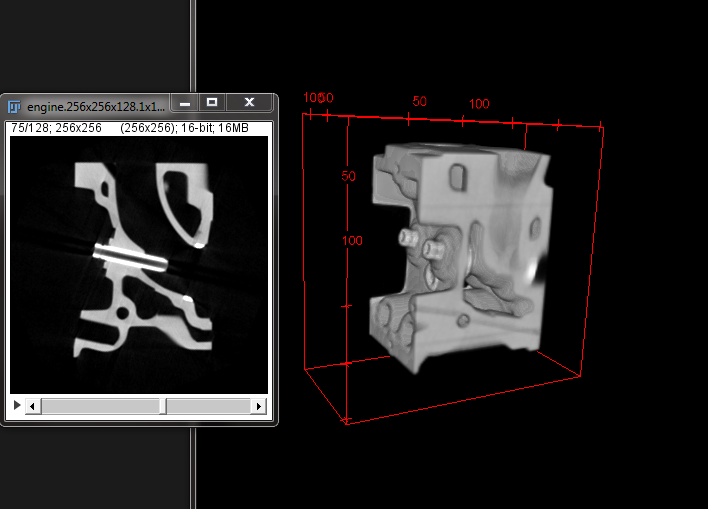
\includegraphics[scale=0.4]{engine.png}\\
\textit{L'objet ENGINE sous fiji}
\end{center}

\paragraph{} Cependant, je n'arrive pas à obtenir un fichier stl fonctionnel. En effet, même si celui ci pèse 226 Mo après exécution de mon algorithme, rien ne s'affiche lorsque je l'ouvre dans un logiciel de création 3D ou dans MeshLab. Il doit y avoir une erreur dans mon code que je n'arrive pas à déceler.

\vspace{3cm}
\section*{Annexe - Code}


\end{document}